\documentclass[a4paper]{article} %,twoside
\usepackage[english]{babel}
%\usepackage[final,ulem=normalem]{changes}

%%
%% Packages to be used.
%%
\usepackage[utf8]{inputenc}
\usepackage{amsmath,amsfonts,amsthm,amssymb,amscd}
\usepackage{booktabs}
\usepackage{multirow}
%\usepackage{zibtitlepage}
\usepackage{alltt}
\usepackage{algorithm}
\usepackage{algorithmic}
\renewcommand{\algorithmicrequire}{\textbf{Input:}}
\renewcommand{\algorithmicensure}{\textbf{Output:}}

%%
%% PDF / DVI output
%%
\usepackage{color}
\usepackage[pdftex]{graphicx}
\usepackage[pdftex]{thumbpdf}
\usepackage{epstopdf}
\graphicspath{{figures/}}

\usepackage{tikz}
\usetikzlibrary{arrows,calc,decorations.markings,intersections,positioning,shapes.arrows}

\usepackage{caption}
\usepackage{subcaption}

\usepackage{cite}
\usepackage[colorlinks=true]{hyperref}

\usepackage{url}
\usepackage{todonotes}

\usepackage{listings}
\lstset{language=Fortran,
	basicstyle=\small\sffamily,
	columns=fullflexible,
	captionpos=b}

\lstdefinelanguage{tt}{
		basicstyle=\ttfamily}
	
%Remove later, used only for getting todos in the margin
%\setlength{\marginparwidth}{3cm}

%%
%% Special sets.
%%
\newcommand{\N}{\mathbb{N}}
\newcommand{\R}{\mathbb{R}}
\newcommand{\One}{\boldsymbol{1}}


%%
%% Mathematical convenience.
%%
\DeclareMathOperator{\ld}{log_2}
\DeclareMathOperator{\convex}{co}
\newcommand{\half}{\frac{1}{2}}
\newcommand{\Ol}[1]{\mathcal{O}(#1)}
\newcommand{\dual}[1]{#1^\star}
\newcommand{\norm}[1]{\left\|#1\right\|}
\newcommand{\const}{\mathrm{const}\,}
\renewcommand{\d}{\mathrm{d}}

\usepackage{pgfplots}
\usepackage{pgfplotstable}
\pgfplotsset{compat=newest}
\usepackage{booktabs}

\begin{document}

\title{Optimal Control of the Initial Condition for the KS Equation With LibPFASST}
\author{Sebastian Götschel}
\maketitle

\section{Problem setting}


We are considering the 1D Kuramoto-Sivashinsky equation
\begin{equation} \label{eq:KS}
y_t = -y y_x - y_{xx} - y_{xxxx}, \quad x \in \Omega := [0,32\pi]
\end{equation}
with periodic boundary conditions on some time interval $t \in [0,T]$. Given some measured data (in the optimal control setting called \emph{desired state}) $y_d(t,x)$, the aim is to identify an initial condition $y(0,x) = u(x)$ such that the solution $y(t,x;u)$ minimizes the deviation from the desired state. We will often refer to $u$ as the \emph{control}. Put into formula, we want to minimize the \emph{objective functional}
\begin{equation}\label{eq:obj}
J(y,u) := \frac{1}{2}\int_{0}^{T} \int_\Omega (y-y_d)^2 \mathrm{d}x\ \mathrm{d}t + R(u),
\end{equation}
where $R$ is some generic regularization term, e.g., $R(u) = \frac{\lambda}{2} \norm{u}^2$.


\paragraph{Gradient-based optimization.} For the gradient-based methods considered here, the optimization iteration proceeds as 
\begin{align}
u_{k+1} &= u_k + \alpha_k d_k \label{eq:update_u} \\
d_{k+1} &= -\nabla j(u_{k+1})+ \beta_k d_k, \label{eq:update_d}
\end{align}
where $k$ is the iteration number, $\nabla j(u_{k})$ the \emph{reduced gradient}, and $\alpha_k$ some step length for the control update. The parameter $\beta_k$ is used to update the descent direction $d_k$ and determines the type of method (steepest descent for $\beta_k = 0$, various choices for nonlinear conjugate gradient methods).

\paragraph{Computation of the reduced gradient.} Adjoint gradient computation consists of three steps:
\begin{enumerate}
	\item Solve the PDE \eqref{eq:KS} for a given control $u$
	\item Solve the adjoint PDE 
	\begin{equation}\label{eq:adjoint}
		-p_t = p p_x - p_{xx} - p_{xxxx} + (y-y_d), \quad x \in \Omega := [0,32\pi]
	\end{equation}
	with periodic boundary boundary conditions and $p(T,x) = 0$.
	\item Set $\nabla j(u) =  p(0,x) + R'(u)$. 
\end{enumerate}
The source term in eq.~\ref{eq:adjoint} comes from differentiating the objective functional \ref{eq:obj} with respect to the state $y$. If, instead of or in addition to, the difference $y-y_d$ in $[0,T] \times \Omega$ we track some desired final state $y_d^T(x)-y(T,x)$ the terminal condition in the adjoint gets modified to $p(T,x) =  y_d^T(x)-y(T,x)$ to account for this deviation.

For details on PDE-constrained optimization see, e.g., \cite{HinzeEtAl2009,Troeltzsch2010}.

\section{Implementation}


This tutorial example consists of six source files
\begin{itemize}
	\item \lstinline+hooks.f90+ - output residuals during sweeps/PFASST iterations
	\item \lstinline+level.f90+ - interpolation/restriction of solutions
	\item \lstinline+main.f90+ - main program, contains main optimization loop
	\item \lstinline+pf_optimization_1d.f90+ - routines for evaluating objective, gradient, steps size selection
	\item \lstinline+probin.f90+ - define problem parameters
	\item \lstinline+sweeper.f90+ - defines problem equations and optimization quantities
\end{itemize}
as well as
\begin{itemize}
	\item \lstinline+Makefile+
	\item \lstinline+imex.nml+ - specify input parameters for test runs
	\item \lstinline+plot.py+ - helper file to produce figures from npy output.
\end{itemize}

In the following we provide a walkthrough through the main parts of the implementation. For all details you will need to go through the actual source code, though.

\subsection{Encapsulation, sweeper, and controller for optimal control}

The LibPFASST library comes with a special data structure \lstinline|pf_ndarray_oc_t| (file \lstinline|pf_ndarray_oc_encap.f90|) to store solutions as well as a IMEX sweeper \lstinline|pf_imexQ_oc_t| (file \lstinline|pf_imexQ_oc_sweeper.f90|) capable of forward- and backward-in-time IMEX-SDC sweeps.

As the optimal control problem requires state and adjoint solution, PFASST's \lstinline|pf_ndarray_t| is extended to contain two variables stored in \lstinline|yflatarray| and \lstinline|pflatarray|. It provides all the functionality of \lstinline|pf_ndarray_t|, with the functions taking an optional \lstinline|flag| argument specifying on which component to operate on (\lstinline|flag==1| operates on \lstinline|yflatarry|, \lstinline|flag==2|  on \lstinline|pflatarry|, and \lstinline|flag==0| on both).

Similarly, the optimal control sweeper provides the same functionality as the standard IMEX sweeper \lstinline|pf_imex_sweeper_t|, again with a \lstinline|flag| argument for the function specifying the component and thus forward or backward sweeps (or both).

Finally, for running PFASST routines like \lstinline|pf_predictor_oc|, \lstinline|pf_pfasst_block_oc| or \lstinline|pf_vcycle_oc| are provided in \lstinline|pf_parallel_oc.f90|. These routines are similar to the standard PFASST functions in \lstinline|pf_parallel.f90|, but adapted to the optimal control setting (e.g., sweeping backwards on the adjoint).

In most cases, the user should not need to edit these library files to solve application problems.

\subsection{The optimization loop}

Besides setting up PFASST and allocating data structures for various quantities used during the optimization, the main part of solving the optimal control problems happens in the optimization loop in \lstinline|main.f90|, see Listing~\ref{lst:optloop}.

\begin{lstlisting}[frame=tb,caption={Most important parts of the optimization loop from \lstinline|main.f90|},label=lst:optloop]
do k=1,max_opt_iter
	if (k .eq. 1) then
		call evaluate_objective(...)
	 else
		objective=objectiveNew ! from step size selection/linesearch
	end if
	
	call mpi_allreduce(objective, globObj, 1, MPI_REAL8, MPI_SUM, pf%comm%comm, ierror)
	if (globObj < tol_obj) exit ! leave loop

	if (k .eq. 1) then   ! in later iterations, this is done in linesearch
		call evaluate_gradient(...)
	end if
	
	 ! compute gradient norms
	globL2NormGradSq = sum(gradient**2)*Lx/dble(nvars(pf%nlevels))
	globLinftyNormGrad = maxval(abs(gradient))
	
	if (sqrt(globL2NormGradSq) < tol_grad) exit
	
	! determine new search direction, here: steepest descent
	beta = 0.0_pfdp
	searchDir = -gradient + beta*prevSearchDir
	
	! line search for step size selection
	call armijo_step()
	
	if (stepTooSmall) exit
end do
\end{lstlisting}
%
Algorithmic parameters like \lstinline|max_opt_iter| or \lstinline|tol_grad| are defined in \lstinline|probin.f90| and can be set via command line parameters or an \lstinline|*.nml| file. The main work happens in the functions \lstinline|evaluate_objective| and \lstinline|evaluate_gradient| from \lstinline|pf_optimization_1d.f90|, where state and adjoint equations are solved, the objective functional gets evaluated and the gradient assembled. Only in the first optimization iteration these are called directly; in the following iterations they get called during linesearch (e.g., \lstinline|armijo_step|).

Solving the state equation by PFASST is done in \lstinline|evaluate_objective|, and is shown in excerpts in Listing~\ref{lst:evalobj}.
\begin{lstlisting}[frame=tb,caption={\lstinline|evalute_objective| from \lstinline|pf_optimization_1d.f90|},label=lst:evalobj]
subroutine evaluate_objective(...)
	! ...
	! set initial condition
	q1%yflatarray = ctrl
	call pf%levels(pf%nlevels)%q0%copy(q1, 1) 
	do step = 1, nsteps ! this iterates over all steps this processor computes
		thisstep = (step-1)*pf%comm%nproc + pf%rank  
		! this is the 'true' time step we are computing 
		! i.e., this processors time interval in this step
		! is [thisstep*dt, (thisstep+1)*dt]
		
		! use PFASST to solve on this block of time steps, i.e., every processors computes 
		! their time step in parallel, exchanging data to transmit
		! initial conditions on the time intervals
		pf%state%pfblock = step    
		call pf_pfasst_block_oc(pf, dt, step*pf%comm%nproc, .true., 1, step=thisstep)
		
		! evaluate objective functional for all quadrature nodes
		do m = 1, nnodes
			call objective_function(...)
		end do
		! integrate objective functional 
		objective = ...
		
		! copy/broadcase qend to q0 for next step
		if( step < nsteps ) then
			call pf%levels(pf%nlevels)%qend%pack(...)   
			call pf_broadcast(...)
			call pf%levels(pf%nlevels)%q0%unpack(...)   
		end if
	end do
	
	! L2(Omega) control norm
	L2NormCtrlSq = sum(ctrl**2)*Lx/dble(nx)
    objective = 0.5*objective + 0.5*alpha*L2NormCtrlSq
end subroutine evaluate_objective
\end{lstlisting}
The main difference to the other Tutorial examples, where a single PDE is solved only once, is, that we cannot use the usual PFASST controller, but have assign blocks of time steps to processors by hand as well as record the solution values in order to solve the adjoint equation backward in time. There, the processors need to solve the specified time steps for which they have the state equation's solution, thus avoiding costly communication as well as memory issues, as every processor only has to store the values it actually needs.

The \lstinline|evaluate_gradient| is similar, and consists of solving the adjoint and constructing the gradient. As the gradient requires the value of the adjoint at $t=0$, the first processor broadcasts this solution to the other processors, see Listing~\ref{lst:evalgrad}. This broadcast could be left out when it is ensured that only the first processor updates the control (i.e., the initial condition); this modification is left as an exercise for the reader.

\begin{lstlisting}[frame=tb,caption={Excerpt of \lstinline|evalute_gradient| from \lstinline|pf_optimization_1d.f90|},label=lst:evalgrad]
if(pf%rank == 0) then
	! gradient is adjoint at t0 (plus regularization term derivative = alpha*ctrl)
	! pack away on rank 0
	call pf%levels(pf%nlevels)%q0%pack(pf%levels(pf%nlevels)%send, 2)
end if
! broadcast
call pf_broadcast(pf, pf%levels(pf%nlevels)%send, pf%levels(pf%nlevels)%mpibuflen, 0)
! everybody sets gradient (actually this could be skipped, only rank 0 needs initial condition)
gradient = pf%levels(pf%nlevels)%send
gradient = gradient + alpha * ctrl
\end{lstlisting}

We do not discuss the line search functions \lstinline|armijo_step| and \lstinline|strong_wolfe_step| here. They are rather straightforward implementations of the standard Armijo- and strong Wolfe conditions (see your favorite textbook on nonlinear optimization, e.g., \cite{NocedalWright2006}).

\subsection{Specifying the equations}

During sweeps, the sweeper calls \lstinline|feval| and \lstinline|fcomp| routines, which are defined in \lstinline|sweeper.f90|. Here the equations are specified. We use an IMEX approach, treating $-y_{xx}-y_{xxxx}$ implicitly.

\begin{lstlisting}[frame=tb,caption={Excerpt of \lstinline|feval| from \lstinline|sweeper.f90|},label=lst:feval]
select case (flags) ! are we solving for state or adjoint?
case(1) ! State
	!  Grab the arrays from the encap
	yvec => get_array1d_oc(y,1) ! ( ,1) means get state component
	fvec => get_array1d_oc(f,1)

	! explicit piece: -y y_x
	tmp = -0.5_pfdp*yvec*yvec
	call fft%conv(tmp, this%ddx, fvec)

case(2) ! Adjoint
	!  Grab the arrays from the encap
	yvec => get_array1d_oc(y,1) ! state sol required for rhs (y-y_desired)
	fvec => get_array1d_oc(f,2)
	pvec => get_array1d_oc(y,2)

	! explicit piece: +y y_x
	tmp = 0.5_pfdp*pvec*pvec
	call fft%conv(tmp, this%ddx, fvec)

	! source term from distributed tracking objective
	fvec = fvec + (yvec-this%ydesired(mystep, idx, :))
end select
\end{lstlisting}

Listing \ref{lst:feval} shows an excerpt of the \lstinline|feval| function, specifying the explicit part of the equation. \lstinline|flags| specifies which equation is to be solved, \lstinline|flags==1| is the state equation, \lstinline|flags==2| specifies the adjoint. In the latter, the source term from the distributed tracking type objective enters. The implicit piece is also evaluated using FFT, \lstinline|call fft%conv(yvec,-this%lap-this%lap*this%lap,fvec)|; this does not differ between state and adjoint.

\begin{lstlisting}[frame=tb,caption={Excerpt of \lstinline|fcomp| from \lstinline|sweeper.f90|},label=lst:fcomp]
if (piece == 2) then
	! Apply the inverse operator with the FFT convolution
	call fft%conv(rhsvec,1.0_pfdp/(1.0_pfdp - dtq*(-this%lap*this%lap-this%lap)),yvec)
	fvec = (yvec - rhsvec) / dtq
end if
\end{lstlisting}

The \lstinline|fcomp| function in Listing \ref{lst:fcomp} is similar to the other tutorial examples and has no modifications due to the optimization problem.


\subsection{Helper and convenience functions}

In \lstinline|sweeper.f90| some helper functions specific to the optimization problem can be found. These are, e.g., \lstinline|initialize_ocp| to allocate memory for the desired state, or \lstinline|set_ydesired| to fill the variable with a desired state coming from measurements or artificially generated data. More importantly, functionality to evaluate the objective functional is provided (\lstinline|objective_function(...)|), as well as functions to restrict the desired state (and the computed fine state solution) to coarser levels as required for solving the adjoint.

\section{Numerical example}

Here we show two numerical results, without giving much detail. Please consider \lstinline|imex.nml| for input parameters.

\subsection{Forward solve}

We use the example from \cite{KassamTrefethen2005} and solve the KS equation for $x\in[0,32\pi]$ on the time interval $[0,60]$ using the initial condition $y(0,x) = \cos(x/16)(1+\sin(x/16))$. The solution using 600 time steps and two levels with 3/5 Lobatto nodes and 512/1024 spatial degrees of freedom is shown in Fig.~\ref{fig:KS60}. 

\begin{figure}
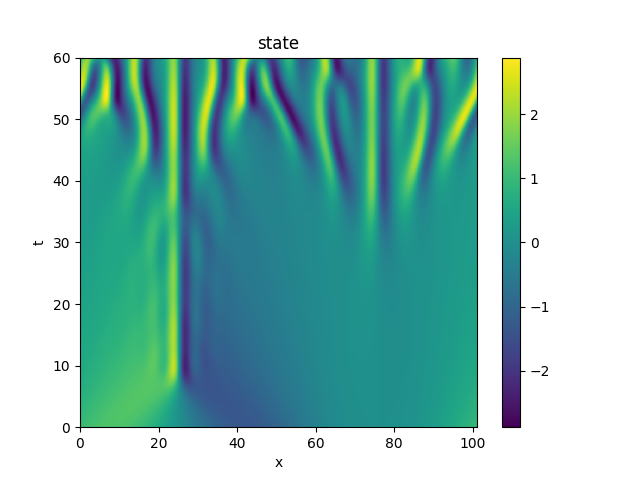
\includegraphics[scale=0.7]{figures/solKS_T60_nstep600_nx1024.png}
\caption{Solution of the KS equation}
\label{fig:KS60}
\end{figure}

\subsection{Identifying the initial condition}

Due to the complicated dynamics, identifying the initial condition is demonstrated on the rather short time interval $[0,1]$, with 100 time steps. The other discretization parameters are as above. We start the optimization with an initial guess $u_0 = 0.75 u_\text{exact}$. The target state is shown in Fig.~\ref{fig:yd}. Fig.~\ref{fig:optprogress} shows the progress of the steepest descent method, while Fig.~\ref{fig:ctrl} shows the computed control (i.e., identified initial condition) as well as the difference of the identified and true initial condition.

\begin{figure}
	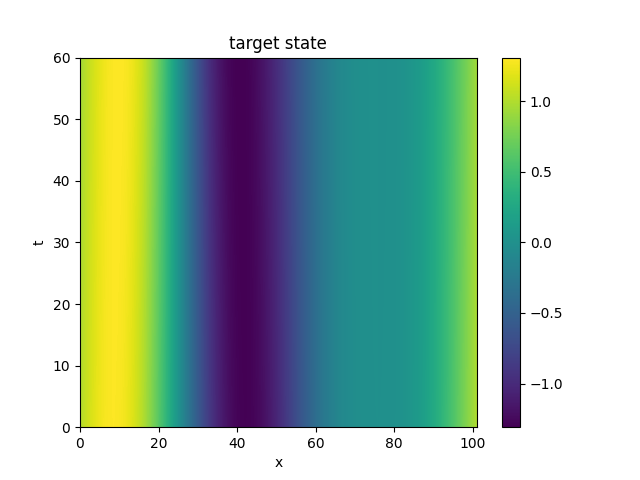
\includegraphics[scale=0.7]{figures/solKS_T1_nstep100_nx1024_yd.png}
	\caption{Target state (KS solution with correct initial condition).}
	\label{fig:yd}
\end{figure}

\begin{figure}
	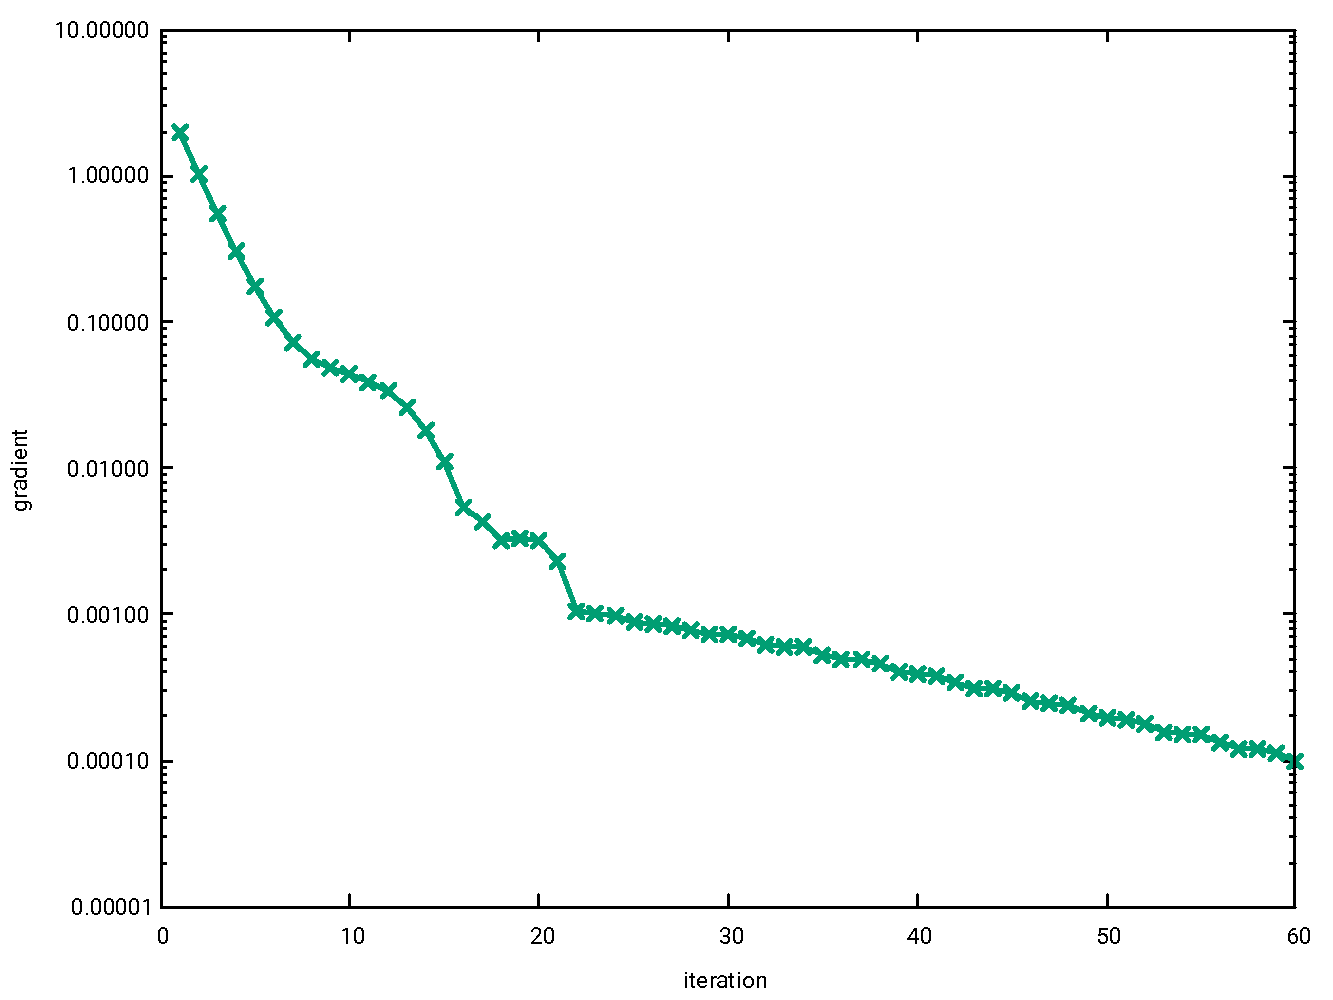
\includegraphics[width=0.5\textwidth]{figures/gradientKS_T1_nstep100_nx1024_u0_075uexact_progress.pdf}
	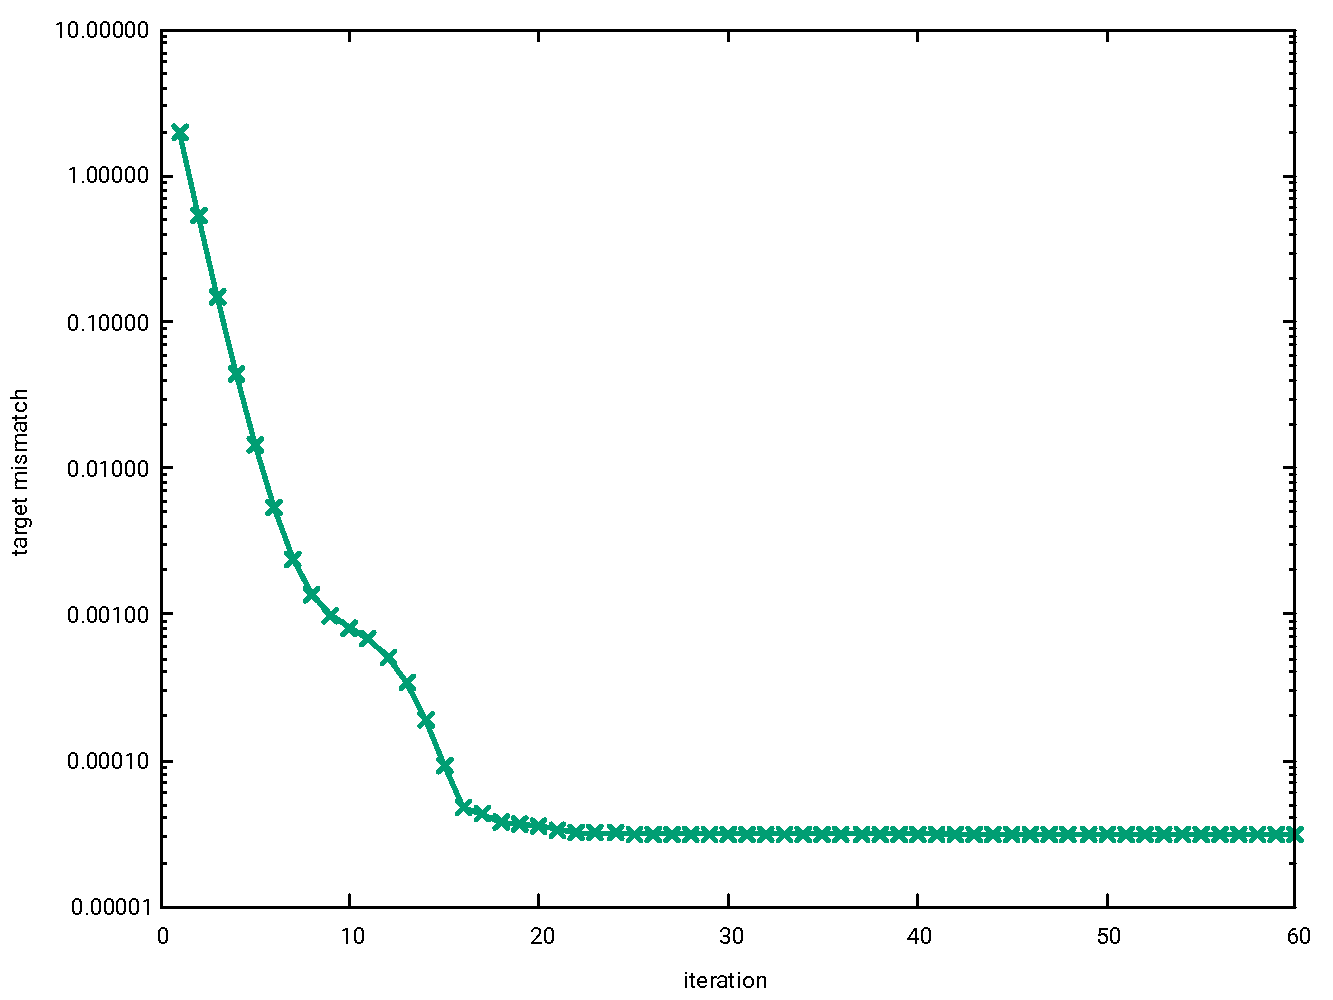
\includegraphics[width=0.5\textwidth]{figures/objKS_T1_nstep100_nx1024_u0_075uexact_progress.pdf}
	\caption{Optimization progress. Left: norm reduced gradient. Right: Target mismatch.}
	\label{fig:optprogress}
\end{figure}


\begin{figure}
	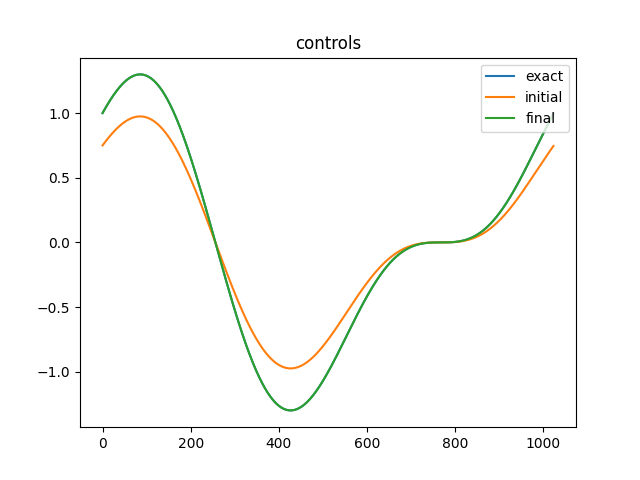
\includegraphics[width=0.5\textwidth]{figures/ctrlKS_T1_nstep100_nx1024_u0_075uexact_progress.png}
	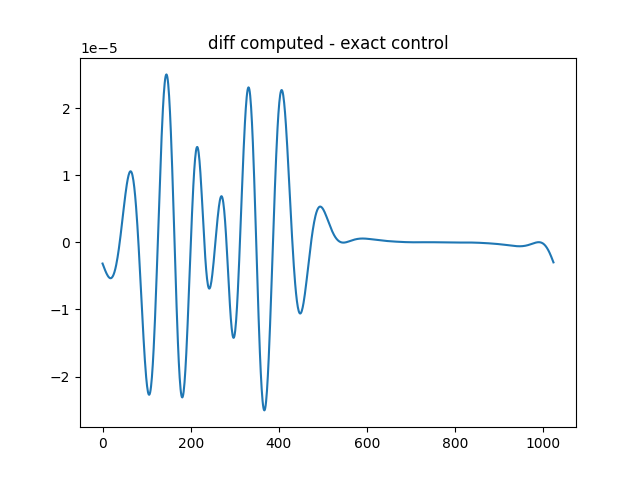
\includegraphics[width=0.5\textwidth]{figures/ctrlKS_T1_nstep100_nx1024_u0_075uexact_diff_final.png}
	\caption{Left: Initial and final control. Right: difference of final to exact control.}
		\label{fig:ctrl}
\end{figure}

\bibliographystyle{plain}
\bibliography{references}

\end{document}
